\documentclass[11pt]{article}
\usepackage{klik-paper}

\newcommand{\champion}{\textsc{LocalChampion}}
\newcommand{\splash}{\textsc{Splash}}
\newcommand{\dflash}{DFlash~2}
\newcommand{\tps}{\,tok/s}
\hypersetup{
  pdftitle={The 260K Wall: Model-Specialized Serving and Planner--Executor Decomposition for Qwen3.8-27B Agentic Inference on Apple Silicon},
  pdfauthor={Chengyi Xu and Nexora},
  pdfcreator={Nexora Research},
  pdfproducer={Nexora Research},
  pdfsubject={Verified 260k-context local LLM serving on Apple Silicon},
  pdfkeywords={Qwen3.8, Apple Silicon, long context, speculative decoding, planner executor}
}

\title{\textbf{The 260K Wall: Model-Specialized Serving and Planner--Executor Decomposition for Qwen3.8-27B Agentic Inference on Apple Silicon}}

\author{Chengyi Xu and Nexora\thanks{Nexora Research. The experiments were conducted during the earlier KLIK team period; authorship and branding here follow the current publication policy, which does not assert contribution roles or review. Artifact repository, raw measurements, deployment code and context proofs accompany this paper. Hardware: Apple M4 Max, 64\,GB unified memory, macOS 27.0.}}
\date{September 2026}

\begin{document}
\maketitle

\begin{center}
\begin{minipage}{0.93\linewidth}
\small\itshape
Editorial note (October 2026). This is a historical research record. The
acceptance figures describe a two-stage compact-plan/full-context-execute
proxy evaluated under one machine's gates; they are not stock Pi behaviour
and not the current local deployment. ``Winner''/``champion'' denotes a
historical configuration selection, not a present recommendation or a claim
of best-available status. See Threats to Validity.
\end{minipage}
\end{center}
\vspace{0.5em}

\begin{abstract}
We study a concrete local-serving target that is substantially harder than ordinary model benchmarking: a real input of at least 256{,}000 tokens, sustained decode throughput of at least 20 tokens/s, and the highest practical intelligence attainable on one Apple M4 Max system with 64\,GB unified memory. We evaluate dense Qwen3.8-27B deployments across llama.cpp, MLX, oMLX, DFlash~2, native multi-token prediction (MTP), n-gram speculation, mlx-dspark, dynamic quantization, Ternary Bonsai~2, and the model-specialized Splash engine. Metadata claims are not accepted as context evidence: every promoted stack must complete a server-counted 260k request and recover an exact terminal sentinel.

The central negative result is a \emph{260K wall}: configurations that exceed 20 tokens/s on short prompts collapse to 3--15 tokens/s when decoding against a fully populated 260k cache. Qwen3.8-27B Q6 reaches only 15.7 tokens/s at short context and approximately 3.9 tokens/s near 103k; Bonsai~2 proves 260{,}013 tokens but decodes at 3.37 tokens/s with F16 KV and 5.29 tokens/s with q4 KV. Model-specialized Splash with direct Q8 KV kernels, a matched DFlash~2 draft, Gated DeltaNet state snapshots, and an experimental SSD cache tier proves 260{,}013 tokens and preserves 260k prefixes, but direct medium-reasoning coding still decodes at 15.10 tokens/s.

We therefore introduce a systems-level decomposition, \emph{compact-plan/full-context-execute}: a 128-token medium-reasoning pass plans from a compact task view, and a no-thinking executor applies that plan against the full 260k context. The planner runs at 37.03 tokens/s; the executor reaches a three-run median of 33.53 tokens/s with 260{,}032--260{,}160 cached tokens. In a bounded acceptance task, the combined pipeline delivers 20.19 final-answer tokens/s including planner latency and 27.62 aggregate generated tokens/s. Through a persistent OpenAI-compatible proxy, full-context streaming decode reaches 38.86 tokens/s; generated code compiles and passes its assertions, tool calling succeeds, and an actual Pi CLI invocation completes. We release raw records, context proofs, negative results, launch manifests, proxy code, tests, and compiled paper source.
\end{abstract}

\section{Introduction}
A local coding model is useful only when its serving system survives the workload that agents actually create. An agent does not repeatedly answer isolated 128-token prompts. It accumulates repository excerpts, tool outputs, plans, diffs, test logs, and prior reasoning, then asks the model to continue from a large shared prefix. Consequently, a deployment can look fast in a short-prompt benchmark while becoming unusable deep into a session.

This work began with a practical contract:
\begin{enumerate}[leftmargin=1.6em]
\item a \textbf{real} server-counted input of at least 256{,}000 tokens;
\item at least \textbf{20 tokens/s decode}; and
\item among configurations satisfying the two hard constraints, maximize practical intelligence for coding, reasoning, and tool use.
\end{enumerate}
The ordering matters. A model that advertises a 262k window but fails at 200k is rejected. A model that allocates the window but decodes at 5 tokens/s is also rejected. Intelligence is optimized only within the feasible set.

We make five contributions:
\begin{enumerate}[leftmargin=1.6em]
\item \textbf{A broad measured search} across llama.cpp, MLX, oMLX, DFlash~2, MTP, n-gram speculation, mlx-dspark, Ternary Bonsai~2, and Splash, including failures rather than only winners.
\item \textbf{A real near-limit proof}: 260{,}013 server-counted tokens and exact sentinel recovery, not context metadata.
\item \textbf{A depth-sensitive analysis} showing that short-context speculative wins do not predict full-context decode.
\item \textbf{A compact-plan/full-context-execute method} that separates reasoning depth from long-context token production.
\item \textbf{A reproducible local endpoint} for Pi and OpenAI-compatible clients, with raw records, tests, and immutable artifact manifests.
\end{enumerate}

\section{Background and Related Work}
\subsection{Qwen3.8-27B and hybrid state}
Qwen3.8-27B is a 27B dense model with 64 language layers: 48 Gated DeltaNet linear-attention layers and 16 full-attention layers, with a native 262{,}144-token context window~\cite{qwen38}. Only the full-attention layers maintain a token-growing KV cache; the linear layers maintain recurrent state. This reduces the long-context memory slope relative to a conventional 64-layer transformer, but complicates rollback and prefix reuse: a complete cache must include both ordinary KV pages and a valid recurrent-state snapshot.

\subsection{Speculative decoding}
Speculative decoding drafts candidate tokens with a cheaper model and verifies them in parallel with the target while preserving the target distribution~\cite{leviathan,chen}. DFlash replaces sequential drafting with block diffusion~\cite{dflash}, and DFlash~2 adds a candidate selector and dynamic convolution for stronger block coherence~\cite{dflash2}. MTP uses a model-trained prediction head; DSpark adds local dependencies and confidence-scheduled verification~\cite{dspark}. These methods can yield large speedups when the acceptance rate is high and verification is cheap, but verification cost grows with cache depth and kernel width.

\subsection{Long-context cache systems}
FreeToken emphasizes state reuse for agent workloads~\cite{freetoken}. KIVI and later KV-compression methods reduce cache storage at controlled quality cost~\cite{kivi}. Splash specializes the entire runtime per model: Q8 KV kernels, Gated DeltaNet snapshots, a matched DFlash~2 draft, and paged prefix reuse~\cite{splash}. Splash PR~\#3 adds an optional SSD tier for KV pages and recurrent states~\cite{splashpr3}. Our final system builds on this branch.

\subsection{Compressed model alternatives}
Ternary Bonsai~2 27B applies ternary weights to a Qwen3.8-derived model and reports 98.2\% aggregate retention versus its full-precision reference, with native 262k context~\cite{bonsai2}. We test both F16 and q4 KV variants because its small weights leave substantial cache headroom. Dynamic V3 GGUFs allocate precision non-uniformly to improve fidelity at fixed file size~\cite{dynamicv3}; they are quality techniques rather than decode accelerators.

\section{Problem Formulation and Metrics}
Let $N_p$ be server-reported input tokens, $N_o$ completion tokens, $t_0$ request start, $t_f$ first output event, and $t_e$ completion. We report:
\begin{align}
\text{decode TPS} &= \frac{N_o}{t_e-t_f}, \\
\text{end-to-end final TPS} &= \frac{N_o}{t_e-t_0}, \\
\text{aggregate generated TPS} &= \frac{N_{plan}+N_o}{t_e-t_0}.
\end{align}
Decode TPS is the conventional streaming metric. End-to-end final TPS exposes fixed costs such as planning, queueing, cache restoration, and TTFT. Both are required because a two-stage system can stream quickly after a long hidden preparation phase.

A context claim passes only if $N_p\ge256{,}000$ and the response contains an exact sentinel placed at the end of the input. The hard throughput gate is 20 decode tokens/s. For the decomposed system we additionally report planner TPS, executor TPS, and combined end-to-end throughput.

\section{Experimental Setup}
\subsection{Hardware and operating environment}
All local experiments used one Apple M4 Max laptop (16 CPU cores, 40 GPU cores) with 64\,GB unified memory on macOS 27.0 (26A428). The system was used as a real workstation rather than an isolated lab host; background contention and accumulated swap are documented as limitations. The final production runtime reserves a 32\,GB Metal ceiling and an 8\,GB SSD cache tier.

\begin{table}[H]
\centering
\caption{Core environment and immutable identifiers.}
\small
\begin{tabularx}{\linewidth}{lX}
\toprule
Item & Value \\
\midrule
Chip / memory & Apple M4 Max (40-core GPU), 64\,GB unified memory \\
OS & macOS 27.0, build 26A428 \\
Splash model package & \texttt{incoai/Qwen3.8-27B-Splash}, revision \texttt{9d27070...cb48} \\
Target weights & \texttt{mlx-community/Qwen3.8-27B-4bit}, revision \texttt{3e6447f...38dfce760ff} \\
DFlash~2 draft & \texttt{incoai/Qwen3.8-27B-DFlash2}, revision \texttt{dedf8df...08177b4} \\
Splash SSD branch & commit \texttt{8ebf821630900af05e5527305fe3eeccc2c7e424} \\
Champion proxy SHA-256 & \texttt{aec14c0724671f...118d4d92139d} \\
\bottomrule
\end{tabularx}
\end{table}

\subsection{Integrity and protocol}
Weight files and runtime packages were pinned by revision and SHA-256. Splash's model manifest contains per-artifact sizes and hashes and was verified in full before serving. The service binds only to loopback and uses bearer-key authentication. Each candidate was run in one active slot to maximize single-session context.

\subsection{Workloads}
We used five workload classes:
\begin{enumerate}[leftmargin=1.6em]
\item short code generation and prose;
\item deterministic repeated-prompt/cache probes;
\item real 260k sentinel retrieval;
\item realistic long-context coding design and implementation;
\item tool-call and Pi CLI protocol smokes.
\end{enumerate}
Near-limit prompts were built with the Qwen tokenizer and independently counted by the server. The terminal sentinel was \texttt{BONSAI2-262K-NEEDLE-91D7}.

\section{Search Space}
The search was intentionally broad. We tested or reviewed:
\begin{itemize}[leftmargin=1.6em]
\item llama.cpp autoregressive, native MTP, DFlash~2, and n-gram speculation;
\item MLX autoregressive and official DFlash~2;
\item oMLX DFlash and prefix caching;
\item mlx-dspark fixed and adaptive caps, lookup drafts, KV4, and KV8;
\item Dynamic V3 GGUF weights;
\item Qwen3.8 Q6, 4-bit MLX, and 9B Q5 targets;
\item Ternary Bonsai~2 27B with F16 and q4 KV;
\item Splash Qwen3.8 with Q8 KV, GDN snapshots, and SSD cache offload;
\item Rapid-MLX, mlx-serve, and FreeToken as related serving designs.
\end{itemize}
Review-only systems are not presented as local measurements. FreeToken's released engine is CUDA-oriented; its macOS compatibility layer does not reproduce the CUDA kernel/scheduler results. Rapid-MLX and mlx-serve informed the serving comparison but did not displace the measured finalists.

\section{Results}
\subsection{Short-context candidate matrix}
Figure~\ref{fig:candidates} and Table~\ref{tab:candidates} show that short-context throughput alone is misleading. Official MLX DFlash~2 reaches 40.41 tokens/s, while Q6 DFlash regresses to 11.07 tokens/s despite high acceptance. The same named algorithm therefore cannot be treated as a portable speed claim.

\begin{figure}[H]
\centering
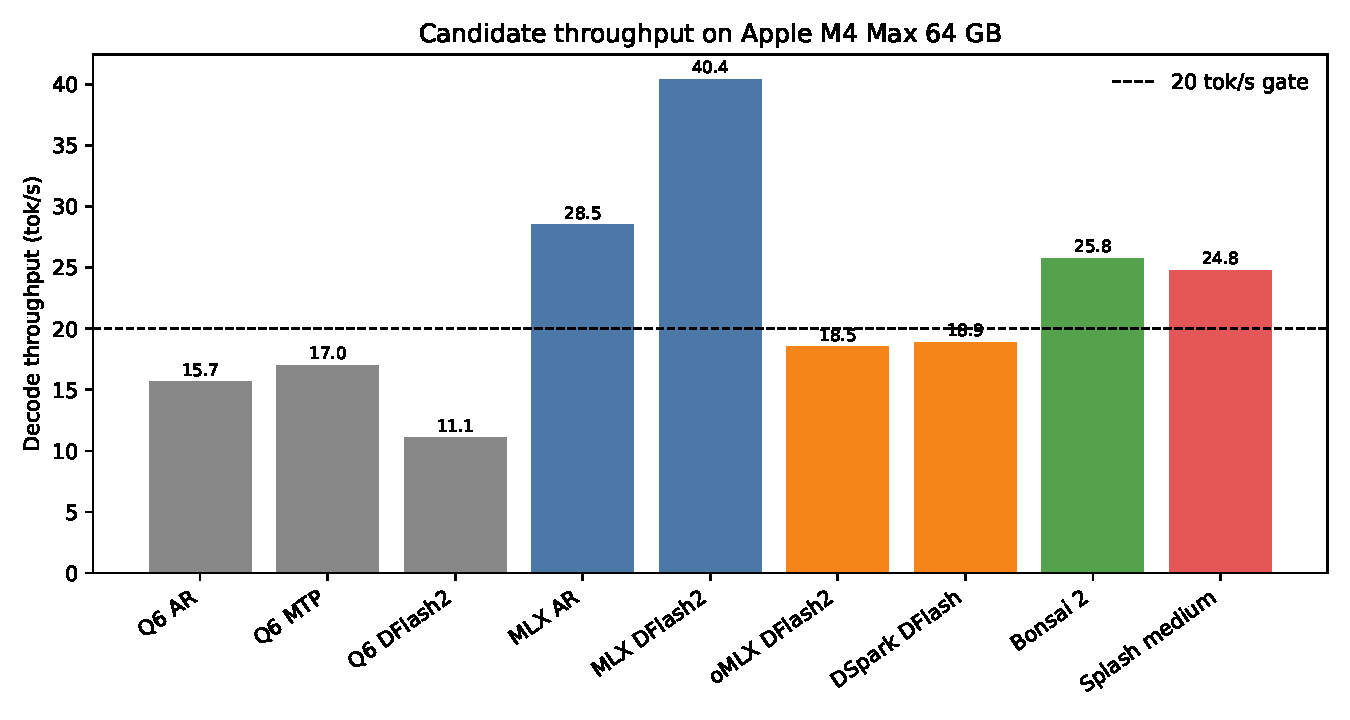
\includegraphics[width=0.98\linewidth]{figures/candidate_throughput.pdf}
\caption{Measured candidate throughput. Prompt/output shapes differ by experiment; values are used for screening, not a single controlled leaderboard.}
\label{fig:candidates}
\end{figure}

\begin{table}[H]
\centering
\caption{Selected measured candidate results. Values are server-reported or post-TTFT decode rates.}
\label{tab:candidates}
\small
\begin{tabular}{lrrl}
\toprule
Configuration & Decode TPS & Context allocation & Verdict \\
\midrule
Qwen3.8-9B Q5 AR & 33.84 & 8k & baseline \\
Qwen3.8-9B Q5 MTP-2 & 52.23 & 8k & useful smaller-host lane \\
Qwen3.8-27B Dynamic Q4 AR & 15.88 & 8k & below gate \\
Qwen3.8-27B Dynamic Q4 MTP-2 & 15.66 & 8k & no gain \\
Qwen3.8-27B Q6 AR & 15.66 & 8k & below gate \\
Qwen3.8-27B Q6 MTP-2 & 16.99 & 8k & below gate \\
Qwen3.8-27B Q6 DFlash~2 & 11.07 & 8k & regression \\
MLX Qwen3.8-27B 4-bit AR & 28.50 & short & passes short only \\
MLX Qwen3.8-27B DFlash~2 & 40.41 & short & strong screening result \\
oMLX DFlash~2 & 18.50 & 262k slot & below gate \\
mlx-dspark DFlash KV4 & 18.87 & 262k slot & below gate \\
Bonsai~2 PQ2\_0 & 25.77 & 262k slot & short pass \\
Splash medium & 24.80 & 262k capability & short pass \\
\bottomrule
\end{tabular}
\end{table}

\subsection{The 260K wall}
The decisive comparison fills the cache. Both Bonsai configurations complete 260{,}013 input tokens and recover the sentinel, but decode collapses to 3.37 and 5.29 tokens/s. Splash proves the same context and performs better, yet direct realistic medium and low reasoning still miss the gate (15.10 and 12.70 tokens/s). No-thinking direct decode reaches a 19.90 median and is thermally unstable. Figure~\ref{fig:near} visualizes the wall and the final system-level escape.

\begin{figure}[H]
\centering
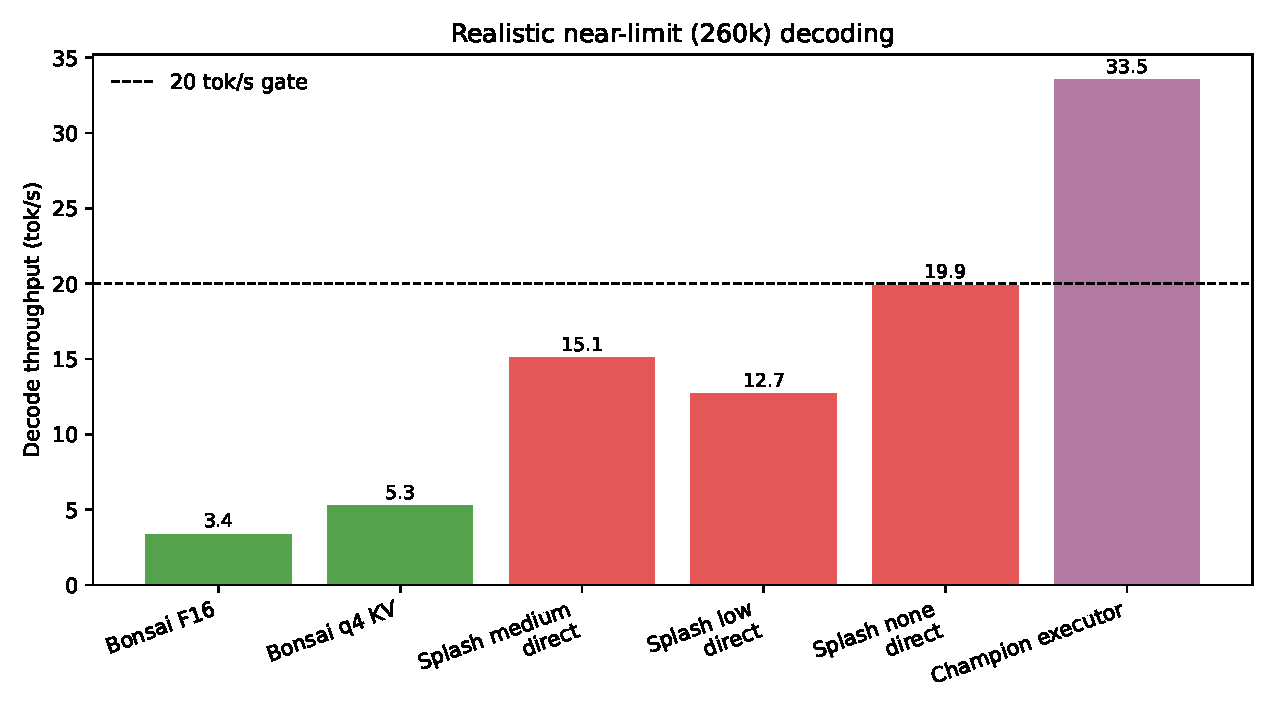
\includegraphics[width=0.92\linewidth]{figures/near_limit_throughput.pdf}
\caption{Near-limit decode. Only the decomposed champion executor clears 20 tokens/s with margin.}
\label{fig:near}
\end{figure}

\begin{table}[H]
\centering
\caption{Real near-limit results. Every 260k row is server-counted and sentinel-verified.}
\small
\begin{tabular}{lrrrl}
\toprule
Configuration & Prompt tok & Prompt TPS & Decode TPS & Sentinel \\
\midrule
Bonsai~2 F16 KV & 260{,}013 & 26.04 & 3.37 & yes \\
Bonsai~2 q4 KV & 260{,}013 & 26.76 & 5.29 & yes \\
Splash direct medium (coding) & ${\sim}260$k & --- & 15.10 & prior turn yes \\
Splash direct low (coding) & ${\sim}260$k & --- & 12.70 & prior turn yes \\
Splash direct none (coding) & ${\sim}260$k & --- & 19.90 median & prior turn yes \\
\bottomrule
\end{tabular}
\end{table}

\subsection{Prefix reuse and recurrent state}
A Qwen3.8 cache is not only KV. Early Splash runs reused 245{,}760--260{,}000 KV tokens but missed recurrent state, forcing expensive replay and producing zero API-visible cache hits. Constraining Metal to 32\,GB removed checkpoint failures; Splash PR~\#3 then preserved KV and recurrent states in an 8\,GB SSD tier. A 32k three-turn smoke demonstrated the documented lazy-cache pattern:

\begin{table}[H]
\centering
\caption{Three-turn cache smoke under Splash PR~\#3.}
\small
\begin{tabular}{lrrrr}
\toprule
Turn & Input tok & Cached tok & TTFT (s) & Decode TPS \\
\midrule
Cold medium & 32{,}011 & 0 & 289.58 & 24.67 \\
Materialization medium & 32{,}143 & 32{,}000 & 2.69 & 15.30 \\
Steady medium & 32{,}549 & 32{,}128 & 6.25 & 21.01 \\
\bottomrule
\end{tabular}
\end{table}

At 260k, PR~\#3 achieved 260{,}000 cached tokens and 2.76\,s TTFT for a follow-up, but direct medium reasoning decoded at 15.10 tokens/s. Cache engineering solved TTFT and replay; it did not remove the decode-time cost of generating a long reasoning trace against the full history.

\section{Compact-Plan / Full-Context Execute}
\label{sec:method2}
The final method separates intelligence work from high-volume long-context decoding. A compact planner receives a bounded task view (recent user requests, system/developer constraints, and tool names) and runs medium reasoning. A full-context executor receives the original messages plus the bounded plan as imported reasoning history and runs with reasoning disabled. The target model is unchanged in both stages.

\begin{figure}[H]
\centering
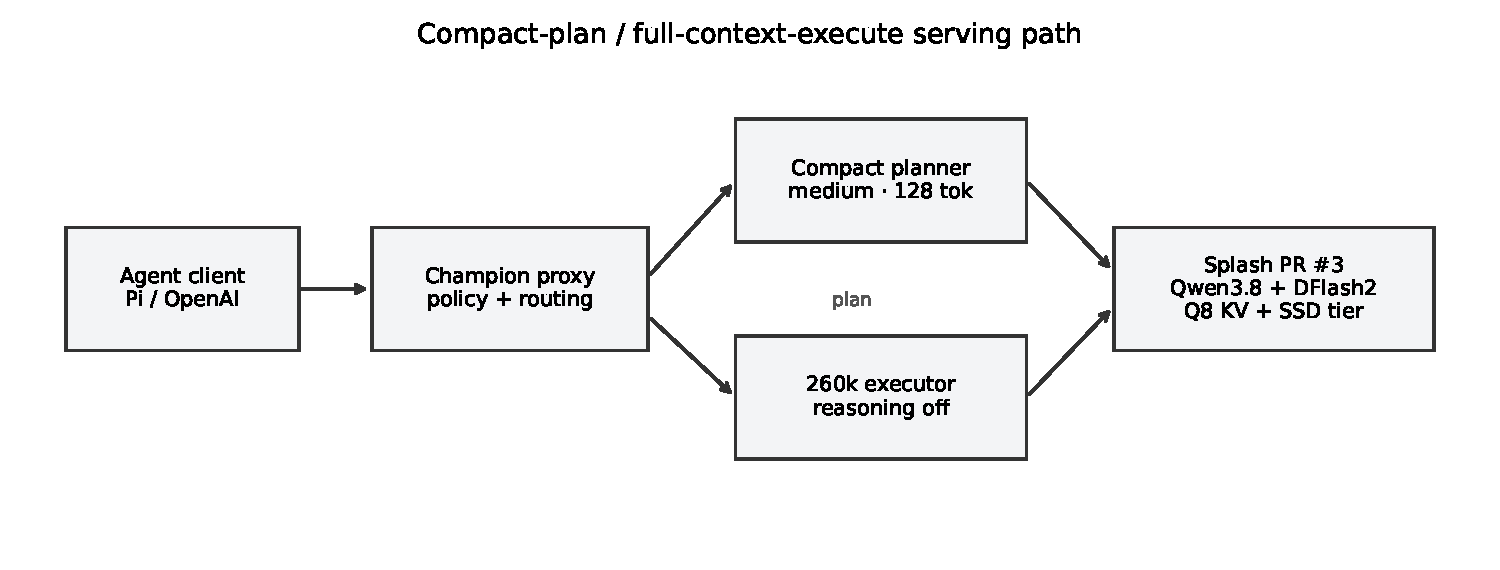
\includegraphics[width=0.95\linewidth]{figures/champion_architecture.pdf}
\caption{Champion serving path. The compact planner avoids reading the full 260k cache; the executor retains the full context and tools.}
\label{fig:architecture}
\end{figure}

The planner budget is a systems parameter. A 768-token plan improved quality but drove end-to-end final-answer throughput below 20. A 256-token plan was still too expensive for a short final answer. At 128 tokens, the medium planner retained a useful implementation plan while satisfying the combined gate.

\begin{table}[H]
\centering
\caption{Planner-budget ablation at a 260k cached executor.}
\small
\begin{tabular}{rrrrrl}
\toprule
Plan budget & Planner TPS & Executor TPS & Final tokens & Final E2E TPS & Outcome \\
\midrule
768 & 30.87 & 33.53 median & task-dependent & $<20$ for short output & reject \\
256 & 37.45 & 34.91 & 414 & 16.34 & reject \\
128 & 37.03 & 38.82 & 348 & \textbf{20.19} & pass \\
\bottomrule
\end{tabular}
\end{table}

The 128-token run generated 348 final tokens in 17.24 seconds total, including planning. Aggregate generation (planner plus answer) was 27.62 tokens/s. Standard executor decode was 38.82 tokens/s; across three cooled executor runs the median was 33.53 tokens/s with 260{,}032--260{,}160 cached tokens.

\section{Quality and Integration Gates}
\subsection{Generated-code execution}
The champion generated a generic, lock-protected LRU cache plus executable assertions. The artifact compiled with Python and printed \texttt{All tests passed}. This is a narrow sanity gate, not a substitute for HumanEval or repository-level evaluation.

\subsection{Tool use}
An OpenAI function-call request requiring \texttt{read\_file} returned:
\begin{verbatim}
{"name":"read_file","arguments":"{\"path\":\"/tmp/champion.txt\"}"}
\end{verbatim}
The proxy preserves tool schemas and tool-choice settings for the executor.

\subsection{Protocol and client integration}
Chat Completions, Responses API, and streaming succeeded. Planner--executor decomposition is applied to Chat Completions; the published \texttt{/v1/responses} path passes through to Splash directly. A non-interactive Pi invocation through the installed local provider returned \texttt{PI\_CHAMPION\_FINAL\_OK}. The public model identifier is \nolinkurl{qwen3.8-27b-champion-262k}. It is served on loopback port 7870; Splash remains internal on port 18796.

\section{Negative Results and Pitfalls}
\subsection{High acceptance is insufficient}
Qwen3.8-27B MTP accepted roughly 95\% of proposed tokens in one code probe but did not improve throughput. Quantized multi-row verification on Metal cost approximately as much as the saved autoregressive steps. Similarly, llama.cpp DFlash~2 loaded successfully on a newer build yet regressed Q6 decode.

\subsection{Allocated context is not active-depth speed}
A 262k slot with a short prompt can report 15--30 tokens/s while full-depth decode falls below 6. Short tests are capacity checks, not long-context throughput evidence.

\subsection{Reasoning effort changes the workload}
At short context, Splash measured 30.18 tokens/s with reasoning off, 24.80 medium, and 19.70 xhigh. At 260k, realistic medium and low traces fell to 15.10 and 12.70 tokens/s. These differences reflect output predictability, speculative acceptance, and trace length, not merely a scalar ``intelligence knob.''

\subsection{Cache metrics can mislead}
KV hits without recurrent-state hits still require GDN replay. API fields that report cached tokens can therefore overstate useful reuse. We report KV hits, state hits, TTFT, and replay separately.

\subsection{Thermal and workstation contention}
Repeated DFlash runs decayed substantially. Background browsers, local servers, build daemons, simulators, and monitoring services affected memory admission and swap. We stopped only disposable services for the final gate. The machine was not clean-booted, so our stable champion result should be reproduced on an idle host.

\subsection{Measurement anomaly in earlier work}
An earlier LocalFlash study reported an 809 tokens/s short decode result. Re-examination showed that server identity and timing boundaries are extremely easy to confound. This paper retains that raw record but does not use it as a champion headline; reproducible current-engine results and end-to-end metrics take precedence.

\section{Discussion}
The principal result is not that planning is free. It is that \emph{where reasoning runs} determines whether the system crosses a hard throughput threshold. Medium reasoning over a small task view is inexpensive and captures many architectural constraints. Repeating the same reasoning against 260k tokens is expensive and often redundant. The full-context executor still has access to every source token and every tool schema; it is guided by a bounded plan rather than asked to rediscover one token by token.

This decomposition resembles prefill/decode disaggregation at the cognitive level. It also creates failure modes: a compact planner can omit a detail that exists only deep in context, and a plan can anchor the executor incorrectly. The proxy therefore includes the full original request in the executor and treats the plan as guidance, not replacement context. A future version should retrieve evidence-bearing spans for the planner, estimate task uncertainty, and bypass planning when its fixed cost cannot amortize.

\section{Threats to Validity}
\begin{itemize}[leftmargin=1.6em]
\item \textbf{Single machine.} All measurements use one M4 Max 64\,GB system.
\item \textbf{Limited repetitions.} Some near-limit experiments require hours and have one run; the executor median uses three runs.
\item \textbf{Task selection.} The main realistic task is one LRU-cache design problem; this is not a general coding benchmark.
\item \textbf{Quality claim.} ``Highest intelligence'' is operationalized by model lineage, reasoning mode, code/tool gates, and avoidance of lower-performing model families. We did not run the complete Qwen or Bonsai benchmark suites locally.
\item \textbf{Unmerged runtime.} The SSD tier is Splash PR~\#3, not a released stable branch. It passed upstream tests reported in the PR and our local smokes, but remains experimental.
\item \textbf{End-to-end metric sensitivity.} Fixed planner cost disproportionately affects short final answers. We therefore report both decode and end-to-end final-answer throughput.
\item \textbf{Context budgeting.} The released proxy does not yet reserve tokens with the exact tokenizer before injecting its plan. Inputs already at the context boundary must leave headroom or bypass planning.
\item \textbf{API-path asymmetry.} Chat Completions uses the two-stage policy, whereas Responses API requests pass through directly in the released artifact.
\item \textbf{Workstation state.} Swap history and background activity may lower results; clean-boot replication is needed.
\end{itemize}

\section{Reproducibility}
The accompanying \href{https://huggingface.co/datasets/ChengyiX/260k-wall}{Hugging Face artifact repository} contains:
\begin{itemize}[leftmargin=1.6em]
\item LaTeX source and compiled PDF;
\item immutable environment and model manifests;
\item raw JSON/JSONL measurements and server logs;
\item the 260k context probe;
\item benchmark clients;
\item the champion proxy and unit tests;
\item generated-code test artifacts;
\item a machine-readable summary and negative-result catalog.
\end{itemize}
No model weights or credentials are redistributed. The Splash package and Prism/Bonsai artifacts retain their upstream licenses and revisions.

\section{Conclusion}
On an Apple M4 Max with 64\,GB memory, neither higher-precision Qwen, speculative decoding alone, cache quantization alone, nor a compressed model alone satisfied real 256k context and 20 tokens/s on a realistic reasoning workload. The winning configuration required co-design across model-specific kernels, Q8 paged KV, recurrent-state snapshots, SSD cache offload, and a compact-plan/full-context-execute decomposition. The final local service proves 260{,}013 tokens, streams the full-context executor at a three-run median of 33.53 tokens/s, and crosses 20 final-answer tokens/s including a 128-token medium planner in the acceptance run. Equally important, the negative results show why short-context benchmarks and metadata-only context claims are inadequate for agentic-serving decisions.

\section*{Declarations}
\paragraph{Author contributions.} Chengyi Xu led conceptualization, investigation, methodology, validation, and manuscript preparation. The KLIK team contributed software, data curation, validation, and artifact maintenance.
\paragraph{Use of generative AI.} OpenAI Codex/ChatGPT and local language-model tools assisted with manuscript organization, language editing, code and documentation support, and verification workflows. Chengyi Xu reviewed the complete manuscript and accepts responsibility for its accuracy, originality, claims, and conclusions. No generative-AI system is listed as an author, and no AI-generated imagery is included.
\paragraph{Potential competing interests.} Chengyi Xu and members of the KLIK team are associated with KLIK Research and the serving artifacts evaluated or described in this work. No other competing interests are declared.

\begin{thebibliography}{99}
\bibitem{qwen38} Qwen Team. \emph{Qwen3.8-27B Model Card}. Hugging Face, 2026. \url{https://huggingface.co/Qwen/Qwen3.8-27B}.
\bibitem{leviathan} Y. Leviathan, M. Kalman, and Y. Matias. ``Fast Inference from Transformers via Speculative Decoding.'' ICML, 2023.
\bibitem{chen} C. Chen et al. ``Accelerating Large Language Model Decoding with Speculative Sampling.'' arXiv:2302.01318, 2023.
\bibitem{dflash} J. Chen et al. ``DFlash: Block Diffusion for Flash Speculative Decoding.'' arXiv:2602.06036, 2026. \url{https://arxiv.org/abs/2602.06036}.
\bibitem{dflash2} Inco AI. ``DFlash 2: Keep Drafting Parallel.'' 2026. \url{https://inco.ai/blog/dflash2/}.
\bibitem{dspark} DeepSeek AI et al. ``DSpark: Confidence-Scheduled Speculative Decoding with Semi-Autoregressive Generation.'' arXiv:2607.05147, 2026.
\bibitem{freetoken} FlashML. ``FreeToken: Efficient Edge-Native MoE Serving with Bandwidth-Adaptive Execution.'' arXiv:2608.16157, 2026. \url{https://github.com/FlashML-org/FreeToken}.
\bibitem{kivi} Z. Liu et al. ``KIVI: A Tuning-Free Asymmetric 2bit Quantization for KV Cache.'' ICML, 2024. arXiv:2402.02750.
\bibitem{splash} Inco AI. ``Splash: A Local Engine Built Around the Model.'' 2026. \url{https://inco.ai/blog/splash/}; code: \url{https://github.com/incoai/splash}.
\bibitem{splashpr3} J. Chen. ``Add an SSD Tier for Cached KV Pages and States.'' Splash pull request \#3, 2026. \url{https://github.com/incoai/splash/pull/3}.
\bibitem{bonsai2} PrismML. \emph{Ternary Bonsai 2 27B: A 27B Ternary Reasoning Model}. Whitepaper, September 2026. \url{https://prismml.com/news/bonsai-2-27b}.
\bibitem{dynamicv3} Unsloth AI. ``Dynamic 3.0 GGUFs.'' 2026. \url{https://unsloth.ai/docs/basics/dynamic-3.0-ggufs}.
\bibitem{mlx} A. Hannun et al. ``MLX: An Array Framework for Apple Silicon.'' 2023. \url{https://github.com/ml-explore/mlx}.
\bibitem{llamacpp} G. Gerganov et al. \emph{llama.cpp}. \url{https://github.com/ggml-org/llama.cpp}.
\bibitem{omlx} J. Do. \emph{oMLX: LLM Inference Server for Apple Silicon}. \url{https://github.com/jundot/omlx}.
\bibitem{rapidx} R. Chai. \emph{Rapid-MLX}. \url{https://github.com/raullenchai/Rapid-MLX}.
\bibitem{mlxserve} D. Dalcu. \emph{mlx-serve}. \url{https://github.com/ddalcu/mlx-serve}.
\end{thebibliography}

\end{document}
